\subsection{Tính toán đường đi tốt nhất cho từng cặp đối cực}
Sau khi tìm thấy tất cả các cặp đối cực, đường dẫn sẽ được tạo cho từng cặp với khoảng cách tương đối là $d_x$ giữa các đường đi, $d_x = n \ell\cos{(\frac{\psi}{2})}$. 
Đối với một cặp đối cực, các đường đi được thiết kế song song với một cạnh của đa giác đi qua một trong các đỉnh của cặp đối đỉnh, còn được gọi là đường cơ sở, Đỉnh trên đường cơ sở được gọi là đỉnh bắt đầu và đỉnh còn lại được gọi là đỉnh kết thúc. Mỗi cặp đối cực có hai đường cơ sở tương ứng với hai hướng cho các đường đi như trong Hình.\Ref {fig:SW1}.

Để xây dựng đường đi bao phủ gồm các đoạn back and forth, các điểm tham chiếu vào một đường dẫn  bằng cách cho các đường đi kể trên giao nhau với đa giác Q. Thuật toán yêu cầu đầu vào là đa giác Q, đỉnh ban đầu B, một đỉnh liền kề có tên $B_{mate}$, và đỉnh đối với đỉnh B được đặt tên là A và khoảng cách giữa các đường đi là $d_x$ đã được định nghĩa bên trên.Đầu tiên, một đường đi L sẽ được tạo, song song với cạnh $( B,B_{mate}$) và phải dịch chuyển vuông góc về phía A (hướng quét) bằng cách bù, $\Delta_{init} = \dfrac{dx}{2}$

    \begin{figure}[H]
        \centering
        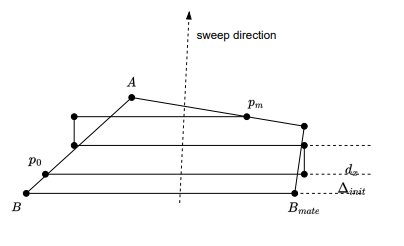
\includegraphics[width=0.7\textwidth]{chapter4/image/anh5.png}
        \caption{Xây dựng đường đi }
        \label{fig:anh5}
    \end{figure}

Số lượng đường đi là tối thiểu nếu RCPP chọn các đường đi song song với đường cơ sở với khoảng cách tối thiểu đến đỉnh kết thúc. RCPP với các tiêu chí như vậy để chọn hướng đường đi được gọi là RCPP tối ưu, được ký hiệu là \emph{Op-RCPP}. Các đường đi song song với đường cơ sở khác được gọi là RCPP không tối ưu, được ký hiệu là \emph{nonOP-RCPP}. Như minh hoạ trong Hình. \ref{fig:SW1}, đỉnh bắt đầu là $C$ và cặp đối cực là $(A,C)$. Hai đường cơ sở đi qua đỉnh $C$ là $CD$ và $CB$ với khoảng cách tương đối là $h_1$ và $h_2$ tương ứng với đỉnh kết thúc $A$. Để đạt được số lượng đường đi ít nhất, khoảng cách tương đối giữa đỉnh kết thúc và đường cơ sở phải nhỏ nhất. Trong ví dụ này, vì $h_1<h_2$, đường đi có số đường nhỏ nhất được đặt song song với $CD$.

\subsection{Chọn một đường đi tối ưu từ tất cả các đường đi của các cặp đối cực}
Biểu thị $pair$ là một tập hợp các cặp đối cực của đa giác. Giả sử rằng mỗi cặp đối mã $(i,j)\in pairs$ có một đường đi tốt nhất với độ dài của nó được ký hiệu là $pth_{ij}$. Gọi $ pth_{ij}^e$ là độ dài của đường đi bao gồm khoảng cách giữa điểm sao $P_s$ và đỉnh $i$, đỉnh $j$ và điểm kết thúc $P_e$. Đường dẫn tối ưu có độ dài $pth_{op}$ được chọn thỏa mãn điều kiện sau:

    \begin{equation}
        pth_{op}=pth_{op}=\min_{(i,j)\in pairs}\{pth_{ij}^{e}\text{\}}
        \label{eq:optimalpath}
    \end{equation}

Thuật toán sẽ thực hiện so sánh tổng quãng đường mà robot đi để bao phủ hết toàn bộ khu vực yêu cầu
trong tệp $pair$. Sau đó sẽ trả về quãng đường đi ngắn nhất thỏa toàn bộ điều kiện của bài toán. Có thể tóm tắt lại thông qua thuật toán \ref{alg:3}

\begin{algorithm}
\caption{Chọn ra đường dẫn tối ưu}
\label{alg:3}
\SetAlgoLined
\KwIn{$V$,\:$p_s$,\:$p_e$}
\KwOut{$fullPath$}
A = findAllAntipodalPairs(V) \;
c = inf\;
\ForEach{ (i,j) $\in$ A}{
    $p = bestPath(V,i,j)\;$
    \If{Cost($p_s,p,p_e$) $<$ Cost($p_e,p,p_s$)}{
    $\tau$ = $\{p_s,p,p_e\}$ \;
    }
    \If{Cost($\tau$) < c}{
        $c$ = Cost($\tau$) \;
        fullPath = $\tau$ \;
     }
}
\end{algorithm}